\chapter{Survey of existing approaches}{``The pessimist complains
  about the wind; the optimist\\expects it to change; the realist
  adjusts the sails.''}{William Arthur Ward}
\label{chap:biblio}

Real-time systems are not new, they have been around for four decades
now. The seminal paper was the work of Liu and
Layland~\cite{liu@jacm73}, which introduced the concepts of processes,
jobs and schedulability. Whereas Manacher~\cite{manacher@jacm67} had
presented the concepts of ``hard real-time'' and ``soft real-time'',
it was Liu and Layland that presented the first major contribution to
the area of real-time systems and who presented the idea of
schedulability and feasibility tests for scheduling. This chapter
presents an introduction to some of the terms and concepts that form
the basis of the work presented in later chapters, as well as a state
of the art for code generation techniques for hard real-time systems.

The first section presents an introduction to real-time tasks (or
threads), their different types and how they differ and their temporal
characteristics. The second section presents an introduction to the
various scheduling techniques currently in use for real-time
systems. Finally, the last section gives an overview of the model
driven code generation approaches that are currently available for
real-time systems. The last section presents some conclusions of the
material introduced.

\section{Real-time tasks}
A real-time task is defined to be any functionality or sequence of
actions that need to be taken by the system under certain temporal
constraints and properties. As stated earlier, a real-time system is
one in which the validity of results depends not only upon the value
computed but also upon the time when those values are available;
real-time tasks are the units of indpendant or co-dependent execution
within the system that may handle different aspects or axes of the
entire computational responsibility imposed upon the system. The idea
of real-time tasks themselves were also first proposed by Manacher
in~\cite{manacher@jacm67}.

An example will serve to best illustrate this point. In a digital
flight control system---the so-called fly-by-wire systems---there
might be one task that reads data from the various atmospheric sensors
such as altimeter, airspeed indicator and gyroscopes. Another task
might be one that reads the command inputs of the pilot (such as the
position of the throttle, joystick and rudder pedals). Finally a third
task would compute the optimum orientation of the various control
surfaces in order to produce the effect desired by the pilot. Each of
these functionalities or tasks may have different temporal constraints
depending upon the characteristics of the sensors, actuators, HCI
requirements such as human response and perception time etc.

Real-time tasks are almost always \emph{recurrent}, i.e., they occur
over and over again during the entire lifetime of a system. Each such
occurrence of a task is called a \emph{job}. In other words, every
time a task is dispatched, it is called a job. The scheduling of tasks
is dependent upon the temporal characteristics of said tasks, the
characteristics of a task that impact on schedulability are shown in
Table~\ref{tab:task_chars}. $C$ is the maximum amount of time one job
of the task may engage in computation if it was executing in
isolation, this is also denoted its WCET (Worst-Case Execution
Time). $T$ is either the \emph{(a)} period of a periodic task or
\emph{(b)} the minimum inter-arrival time for a sporadic task. $I$ or
interference is the amount of time a ready task is not given the
processor because a higher-priority task is executing. $B$ or blocking
time is the amount of time a ready task is not given the processor
because a lower priority task with higher \emph{inherited priority} is
executing (Sec.~\ref{sec:process_based}).

\begin{table}
\centering
\begin{tabular}{|c|l|}
\hline
\textbf{Symbol} & \textbf{Description}\\
\hline
$C$ & Worst-case execution time (WCET)\\
$T$ & Period or minimum inter-arrival time\\
$I$ & Interference time\\
$B$ & Blocking time\\
\hline
\end{tabular}
\caption{Task temporal characteristics}
\label{tab:task_chars}
\end{table}

\subsection{Periodic or time-triggered tasks}
Periodic tasks are those that are dispatched at regular intervals,
called the \emph{period} of the task. The authors of~\cite{sha@rts04}
define periodic tasks as:

\begin{quote}
 \emph{``A task is called periodic if it is time-triggered, with a
   regular release. The length of time between releases of successive
   jobs of task $\tau_i$ is a constant, $T_i$, which is called the
   period of the task.''} 
\end{quote}

In this document, a task is identified using $\tau_i$ for the $i^{th}$
task in a system. Its period is given by $T_i$ and its deadline by
$D_i$. In general, periodic tasks carry out the following
functionalities:

\begin{description}
\item[Control loops:]{In real-time control systems, periodic tasks
  carry out the computation of the \emph{transfer function} that gives
  the output to the actuators as a function of the current and
  previous input from the sensors and the current state of the
  platform;}
\item[Sensor reading:]{In both real-time control and real-time
  information systems such tasks are also used to periodically read
  data from sensors;}
\item[Status displays:]{In real-time information systems such tasks may
  be used to periodically update a status display to provide important
  information to the operator. A typical example might be the update
  of a moving map display associated with a GPS navigation system.}
\end{description}

A timeline representation of a periodic task with a period of $T_p$,
and a runtime of $C_p$ is shown in the lower part of
Fig.~\ref{fig:thread_timeline}. If the first job of $\tau_p$ is at
$t_0$, then its execution finishes at $t_0 + C_p$. Because of the
periodic nature of the task, the second job is dispatched at $t_0 +
T_p$ and finishes $C_p$ time units after its start. The third job
starts at $t_0 + 2T_p$ and the $k^{th}$ job is dispatched at $t_0 +
(k-1)T_p$. Almost all periodic tasks are hard real-time tasks, i.e.,
their deadlines must be respected or the system risks
instability. Thus for a job of $\tau_i$ that is dispatched at $k\times
T_i$, its execution \emph{must} terminate nominally at $k\times T_i +
D_i$, where $D_i$ is its deadline.

\begin{figure}
\centering
\includegraphics[scale=0.6]{figs/thread_timeline}
\caption{Above: Two jobs of a sporadic thread, arriving
  randomly. Below: Three consecutive jobs of a periodic thread,
  arriving at regular intervals.}
\label{fig:thread_timeline}
\end{figure}

\subsection{Aperiodic or event-triggered tasks}
An aperiodic task is defined---rather tersely---in~\cite{sha@rts04}
as:

\begin{quote}
\emph{``A task is aperiodic if it is not periodic''}. 
\end{quote}

A more detailed definition is that aperiodic tasks are those that
may be dispatched as a result of an environmental event or a software
generated event from another task (which may be periodic or
aperiodic itself). An aperiodic task may be a hard or a soft
real-time task. These tasks also have certain temporal constraints
and properties as in the case for periodic tasks.

Thus, for any aperiodic task $T_i$, its WCET or Worst-Case Execution
Time is denoted by $C_i$. It will also have a deadline given by $D_i$,
which specifies that for any aperiodic job dispatched by an event at
time instance $t_1$, the nominal execution of the job in question must
complete at most till time instance $t_1 + D_i$. And whereas a
periodic task must be launched at integer multiples of its
period---$k\times T_i$---an aperiodic task may be dispatched at any
instance of time. Thus, a timeline representation of an aperiodic task
$\tau_i$ is given in the upper part of Fig.~\ref{fig:thread_timeline}.

\subsection{Sporadic tasks}
A sporadic task---again according to~\cite{sha@rts04}---is an
aperiodic task with an upper bound on the load it may impose upon the
system. In other words, a sporadic task is an event-triggered task
with a stipulated and enforced minimum inter-arrival time between
successive dispatches of the task. It is thus a safer version of the
aperiodic task. The inter-arrival time of a sporadic task is denoted
by $T_i$, for the task denoted $\tau_i$. Interestingly, if we assume
the maximum possible load of a sporadic task, it starts behaving like
a periodic task with a period equal to its minimum inter-arrival time.

Associated with a sporadic task is usually an incoming event queue
with a certain size. One of the characteristics of any sporadic task
may be what to do in case of an overflow of the queue; this would be
the case when a burst of dispatching events comes in, overwhelming the
event queue. In the context of this thesis, two ``overload protocols''
are defined for event queues of sporadic tasks:

\begin{description}
\item[Hot Overflow]{this stipulates that an incoming event to an
  already full event queue is rejected, i.e., the \emph{hot} event
  overflows;}
\item[Cold Overflow]{this stipulates that an incoming event to an
  already full queue is inserted at the tail of the queue and the
  event at the head of the queue---the oldest queued event---is
  purged, i.e., the \emph{cold} event overflows.}
\end{description}

\section{Scheduling}
\label{sec:scheduling}
Scheduling of real-time tasks is one of the most important activities
in such a system. Scheduling denotes the ordering of the various tasks
in the system. In a real-time system, such an ordering must take into
account the temporal characteristics---period, type of task whether it
is periodic or aperiodic, inter-arrival time for sporadic, worst-case
execution time etc.---as well as temporal constraints such as the
deadline of each task. A \emph{feasible} schedule in a real-time
system is such that all tasks meet their respective deadlines. A
number of techniques have been developed for the scheduling of
real-time tasks, and below are a number of the most commonly used and
specially the one that is the basis for the work in this thesis.

\subsection{Cyclic executives}
Cyclic executives are one method to create a real-time system with
multiple functions. This type of executive is conceptually simple,
consisting of a single timer callback that runs at the rate of the
fastest function of the system, which is called the \emph{base
  rate}. All other functions are \emph{harmonic} compared to the base
rate, meaning their rates are integral multiples of the base rate. The
timer callback is responsible for calling the procedures that
represent the system functions in accordance with their rates. For
example, if a function $b$ has a rate that is twice that of the base
rate of the system, then it will be called once every second time the
clock interrupt is executed. An example of what such a clock interrupt
handler would look like is shown in Listing~\ref{lst:cyclic_callback}
and a graphical representation of how it is done is shown in
Fig.~\ref{fig:cyclic_exec}.

\begin{figure}
\centering
\includegraphics{figs/cyclic_exec}
\caption{A cyclic executive consists of a timer callback invoking
  procedures in a fixed order}
\label{fig:cyclic_exec}
\end{figure} 

\begin{minipage}{\listingwidth}
\lstset{language=c}
\begin{lstlisting}[label=lst:cyclic_callback, caption=The timer callback
    for a cyclic executive running four separate harmonic tasks]
void clock_tick (int sig, siginfo_t *siginfo, void *context)
{
  static int job = 0;
  job++;
  sensor_a_job();
  if ( job==2 || job==4 ) {
    sensor_b_job();
    data_fusion_job();
  }
  if ( job==4 ) {
    actuator_job();
    job = 0;
  }
}
\end{lstlisting}
\end{minipage}

Data transfer among the various procedures that make up the different
functions of the system is trivial: all data that must be shared among
the various functions is simply put in the heap (global memory), from
where it can be accessed by the various procedures. The question of
concurrency-control or race conditions does not arise because there is
no preemption (as there are no threads). Each procedure will start and
finish its execution without fear of being removed from the processor,
thus there is no chance of a procedure being interrupted while it is
in the middle of making a modification to a global data structure.

A cyclic \emph{schedule} is, however, difficult to
construct~\cite{locke@rts92}. But once it is constructed it needs no
further schedulability analysis, its construction \emph{is} proof of
feasibility~\cite{burns-rtspl}; as long as the execution times of each
procedure invoked by the callback are within bounds for the next one
to start at an appropriate time and for the processing of each timer
callback to finish before the next time the timer callback is
executed. It is also completely deterministic, in that the sequencing
of the various functions is known \emph{\`a priori}. However, it does
suffer from quite a few disadvantages~\cite{locke@rts92}:

\begin{itemize}
\item{Difficult to incorporate sporadic processes;}
\item{Any function with a long computation time (WCET) will need to be
  factorized into a number of smaller functions which will induce
  extraneous dependencies between them;}
\item{A cyclic executive leads to a large number of processor cycles
  that are lost;}
\item{Difficulty in constructing such an executive, specially for
  systems with high utilization~\cite{burns-rtspl};}
\item{Not flexible or amenable to change. Once a system has been
  constructed using this approach, it is very difficult to, e.g., add
  a new function to it, since it necessitates finding a correct call
  sequence that would not break the dependencies between the functions
  and result in a feasible execution;}
\item{In case of an accidental overrun by any task, the entire system
  becomes unstable because a timer interrupt will arrive while the
  previous one is being run, which can cause an avalanche effect.}
\end{itemize}

But the most important disadvantage is the fact that the periods or
rates of all the functions in the system \emph{must} be an integer
multiple of the base rate of the system. However, given these
disadvantages it is important to note that cyclic executives are the
type almost exclusively used in real-time control systems. This is
because they provide a level of determinism that cannot be had with
normal process-based executives (complete operating systems with
schedulers). The \simu real-time development environment from
Matlab~\cite{simulink} generates a cyclic executive and is extensively
used in industry for control system applications such as fly-by-wire
and drive-by-wire applications~\cite{bishop-ctrl}.

\subsection{Process based executives and schedulers}
\label{sec:process_based}
The other alternative for a multiprogramming executive is a
\emph{full-tasking} or process based executive. This is the
traditional approach where an operating system creates multiple,
independent processes, each with potentially multiple threads of
control (with or without preemption). Process based scheduling is made
possible due to the ability of the microprocessor to switch between
different processes very quickly via a \emph{context switch}, where
the contents of the entire register file of the processor are swapped
out to memory and those of another process are loaded into the
processor, giving the process the illusion that it is executing in
isolation with the full resources of the computer at its
disposal. Real-time schedulers can be classified according to two
different categories:

\begin{description}
\item[Preemption:]{Schedulers can be preemptive or
  non-preemptive. Preemptive schedulers can interrupt a task while it
  is being executed via a context switch and place another task on the
  processor. Non preemptive schedulers cannot preempt a task and must
  wait for the task to yield control itself to the scheduler;}
\item[Static/dynamic priorities:]{Static priority schedulers are those
  in which each task is assigned a priority at system initialization
  time and is not changed during the lifetime of the system. Dynamic
  priority schedulers are those in which task priorities change during
  the execution of the system as a function of the various temporal
  characteristics and importance of the task.}
\end{description}

\subsubsection{Fixed Priority Preemptive Scheduler}
The simplest to implement and the most widely-used scheduler in
real-time systems is the Fixed Priority Preemptive Scheduler
(FPPS)~\cite{liu@jacm73, sha@rts04, audsley@rtoss91}. In this
approach, tasks are assigned priorities pre-runtime and remain
static. The scheduler selects the highest priority runnable task at
any given point in time to put on the processor. The Rate Monotonic
Assignment (RMA) is an optimum assignment of priorities to tasks for
an FPPS scheduler, in that if a feasible priority assignment exists
for the given task-set with an FPPS scheduler, the task-set is
schedulable with RMA. The priority assignment is in inverse proportion
to the periods (or inter-arrival time) of tasks. The fastest task has
the highest priority, the slowest task has the lowest priority, i.e.,
for any two tasks if $T_i < T_j$ then $Priority_i > Priority_j$.

\paragraph{Basic schedulability analysis}
Assume that all tasks are independent (no inter-task communication or
synchronization) and hard (no missed deadlines permissible). In the
basic version of the analysis it is assumed that all deadlines are
equal to task periods (or inter-arrival times), $\forall i:D_i =
T_i$. The first commonsense test is that the computation time for all
tasks are less than or equal to their periods, $\forall i:C_i <=
T_i$. The test for schedulability is given by
Eq.~\ref{eq:rma_wo_sync}. This implies a utilization upper bound of
69\% for a large number of tasks. With $C_i/T_i$ in
Eq.~\ref{eq:rma_wo_sync} being the processor utilization of task
$\tau_i$.

\begin{equation}
\label{eq:rma_wo_sync}
\sum_{i=1}^n \bigg(\frac{C_i}{T_i}\bigg) \le n(2^{\frac{1}{n}}-1)
\end{equation}

\paragraph{Response Time Analysis}
A more exact analysis is the Response Time
Analysis~\cite{joseph@tcj86} and~\cite{burns-rtspl} (pp
475---479). The response time of a task is defined as the time between
the dispatch of a job of the task and the successful completion of
that job. If, for a task, the response time can be shown to be less
than the deadline then that task is schedulable.

It is obvious that the response time $R$ for the highest priority task
will be equal to its worst-case execution time. All other tasks will
suffer \emph{interference} from higher priority tasks. In the general
case, for a task $\tau_i$, the response time $R_i = C_i + I_i$. The
form of the equation for the response time of a task is given in
Eq.~\ref{eq:rta_wo_sync}, where $hp(i)$ gives the set of all tasks
with a priority higher than $\tau_i$.

\begin{equation}
\label{eq:rta_wo_sync}
R_i = C_i \ + \sum_{j\in hp(i)} \bigg\lceil\frac{R_i}{T_j}\bigg\rceil C_j
\end{equation}

Since Eq.~\ref{eq:rta_wo_sync} is a fixed-point equation, it can be
solved via a recurrence relation such as the one shown in
Eq.~\ref{eq:rta_rr_wo_sync}. The values of $\omega_i^{n+1}$ are
successively calculated until \emph{(a)} two successive values of
$\omega_i$ are similar and are less than $D_i$ or \emph{(b)} the value
of $\omega_i$ grows larger than $D_i$, in which case this task is not
schedulable.

\begin{equation}
\label{eq:rta_rr_wo_sync}
\omega_i^{n+1}=C_i \ + \sum_{j \in hp(\tau_i)}
\bigg\lceil\frac{\omega_i^n}{T_j}\bigg\rceil C_j
\end{equation}

\paragraph{Communication and synchronization among tasks}
In almost all real-time systems tasks will interact with each
other. Communication among tasks implies shared data buffers protected
via mutexes or semaphores, while synchronization among tasks implies
shared data buffers protected by mutexes or semaphores \emph{and}
condition variables to send asynchronous events. The introduction of
shared buffers and mutexes raises the possibility of
\emph{deadlock}~\cite{levine@sigops03}. Keeping in mind the
safety-critical nature of the software under consideration, deadlocks
and livelocks are unacceptable. The ``Priority Ceiling
Protocol''~\cite{sha@toc90} (or PCP) is a method of implementing
shared buffers and critical sections that completely avoids the issue
of deadlock. It also minimizes to a large extent the ``blocking time''
for tasks, i.e., the time spent by a high priority task waiting for a
shared resource locked by a low priority task. The PCP implies that
every shared resource has a priority associated with it, called its
ceiling priority. The Immediate Ceiling Priority Protocol (ICPP, a
variant of PCP) implies:

\begin{itemize}
\item{Each task has a base priority which is static;}
\item{Each shared resource has a ``ceiling priority'', the maximum of
  the priorities of all tasks that may access it;}
\item{When a task is inside a shared resource, its active priority is
  the maximum of its current active priority and the ceiling priority
  of the resource.}
\end{itemize}

For a system that uses the PCP, the blocking time $B_i$ for any task
$\tau_i$ can be calculated using Eq.~\ref{eq:pcp_block} (Sec. 13.11
of~\cite{burns-rtspl} and~\cite{sha@toc90}), where $usage(k, j) = 1$
if critical section $k$ is used by at least one task with a priority
less than $\tau_j$ and at least one task with a priority greater than
or equal to task $\tau_j$; otherwise $usage(k, j) = 0$. $K$ is the set
of all critical sections and $C_k$ is the WCET of critical section
$k$.
\begin{equation}
\label{eq:pcp_block}
B_j = \max_{k=1}^{K} \Big(usage(k,j)\times C_k\Big)
\end{equation}

This result can be used in both Eqs.~\ref{eq:rma_wo_sync}
and~\ref{eq:rta_wo_sync}. To incorporate it into the Rate Monotonic
Analysis, assume that there are $n$ tasks arranged in increasing
periods; $\tau_1$ is the slowest and $\tau_n$ is the fastest
task. Then the utilization test becomes as shown in
Eq.~\ref{eq:rma_w_sync}, with the summation term the
\emph{interference} from higher priority tasks and $B_j/T_j$ the
\emph{blocking} due to priority inversion by a lower priority task on
a higher priority task. Blocking happens when the lower priority task
inherits the priority of a protected object that is equal to or
greater than the base priority of the higher priority task.
\begin{equation}
\label{eq:rma_w_sync}
\forall j,\ 1 \le j \le n:\ \sum_{i=1}^j
\bigg(\frac{C_i}{T_i}\bigg)+\frac{B_j}{T_j} \le j(2^{\frac{1}{j}}-1)
\end{equation}

Similarly, the PCP result can be incorporated into the Response Time
Analysis by adding the blocking term to the response time equation,
which then becomes Eq.~\ref{eq:rta_w_sync} as given below.
\begin{equation}
\label{eq:rta_w_sync}
\omega_i^{n+1}=C_i + B_i + \sum_{j \in hp(\tau_i)}
\bigg\lceil\frac{\omega_i^n}{T_j}\bigg\rceil C_j
\end{equation}

\subsubsection{Earliest Deadline First Scheduler}
This is an example of a dynamic priority scheduler. This scheduler
puts the task with the nearest deadline on the processor at all
times. Although a detailed discussion of the EDF scheduler is not
given here, note that Liu and Layland gave the utilization upper bound
for this scheduler as 1 in~\cite{liu@jacm73}:
\begin{displaymath}
\sum_{i=1}^N \bigg(\frac{C_i}{T_i}\bigg) \le 1
\end{displaymath}

However, despite this obvious advantage over FPPS, EDF schedulers are
not widely used in industry, the reasons being that an FPPS is much
easier to construct and has a much lesser runtime overhead compared to
an EDF. Under overload conditions, an FPPS is much more predictable as
it will start letting lower priority tasks overrun their deadlines,
compared to an EDF whose behavior is more unpredictable.

\section{Model-driven Approaches}
This section provides an overview of the available model driven code
generation approaches available for software engineering in general
and for the real-time domain in particular.

\subsection{Lustre and SCADE Suite}
Lustre is a synchronous, data flow programming language for reactive
systems~\cite{halbwachs@popl87, halbwachs@ieee91}. The SCADE
Suite~\cite{caspi@sigplan03} is a commercial design environment that
provides a graphical front-end for easily designing Lustre
programs. It is provided by Esterel Technologies and its code
generator (KCG) is certified up to DO-178B Level A, making it an
attractive choice for flight software development. An interesting
history of this approach and a synopsis of the industrial uses it has
found is given in~\cite{halbwachs@memocode05, halbwachs@ieee03}.

Lustre is a synchronous~\cite{halbwachs@ieee03}, data driven (rather
than event driven) and functional language. Inputs are considered as
``flows'', continuously occurring---and possibly changing---values
within a certain domain. These inputs are used to compute output
flows. The language allows the division of programs into different
``nodes'', which are the individual functional units, similar to
subprograms or procedures in an imperative language. Each node has one
or more input flows, and one or more output flows, with the relation
between them defined using discrete equations, e.g., $x = y + z$,
which means \emph{at each instance, step or clock tick k}, $x_k = y_k
+ z_k$. Thus a basic Lustre program is in effect an infinite loop,
this meshes well with control systems because control loops themselves
are infinite and non-terminating over time.

Synchrony, or synchronous processing, assumes that the processing
needed as a response to an environmental stimulus is instantaneous. In
addition, synchronous languages such as Lustre allow for only
deterministic constructs, which results in programs in which internal
actions take place at well-defined times (this is ensured via a cyclic
executive underneath the program). These two features result in
programs that are deterministic from a functional \emph{and} a
temporal viewpoint~\cite{halbwachs@ieee91}. This implicates a
hypothesis that a synchronous program can react to an external event
before another event occurs. Thus synchrony presents programmers a
powerful abstraction which allows them to model their systems at a
higher level, considering only the functional aspect resulting from
the problem domain. If it is possible to check that this hypothesis of
synchrony holds for a system, then these design methods can be brought
to bear on the problem.

The fact that variables in Lustre represent flows coupled with the
fact that designers of control systems are familiar with modeling of
their systems using network operators that transform data flows leads
to a marriage of the synchronous computation and data flow programming
paradigm to give the semantics of Lustre. Because all variables in
Lustre are flows, all boolean, arithmetic and logic operators are also
taken to apply point-wise to elements of the flow. Thus, the
expression ``\texttt{x = \textbf{if} y >= 0 \textbf{then} y
  \textbf{else} -y}'' states that at every step or tick, the value of
$x$ is the absolute value of $y$. In the SCADE Suite tool, this would
be expressed visually as shown in Fig.~\ref{fig:scade_eq} (both taken
from~\cite{halbwachs@ieee03}).

\begin{figure}
\centering
\includegraphics{figs/scade_eq}
\caption{A simple data-flow network}
\label{fig:scade_eq}
\end{figure}

Some Lustre operators that act on flows and which are very useful from
a control systems perspective are the \kw{pre} operator and the $\to$
or \kw{fby} operator. The \kw{pre} operator gives the value of its
argument from the previous cycle. Thus if $X = \{x_0, x_1, x_2,
  \ldots\}$, then $pre(X) = \{nil, x_0, x_1, x_2, \ldots\}$. The
    followed-by operator, \kw{fby} or $\to$, allows correct
    initialization of flows, by avoiding the \texttt{nil} value. If
    $X$ and $Y$ are two flows then $X \to Y$ is a flow which has the
    first value of $X$ at the first cycle, followed by $Y$ at all
    subsequent clock values, i.e., $X \to Y = (x_0, y_1, y_2, y_3,
    ...)$.

Formally, a flow in Lustre is defined as a sequence of values
\emph{and} an associated clock. Since Lustre programs are run on a
cyclic executive, every program has a cyclic behavior, and the clock
of the main node that defines the program is called the \emph{basic
  clock}, it is similar to the \emph{base rate} as defined in the
\simu execution model. Every flow takes its $n^{th}$ value at the
$n^{th}$ time of its clock. Various expressions or nodes can be
defined to be occurring at a different period or frequency by using
boolean flows as clocks for other flows, where the clock defined by
that flow is assumed to be the sequence of times at which said flow
has a value of true. Table~\ref{tab:lustre_clocks} shows a flow C with
the basic clock, whose value is true every time the clock is modulo
2. C' has the clock defined by flow C, and its expression is that it
is initialized to 10 and is doubled at each step, i.e., \texttt{C' =
  10->\textbf{pre}(C')*2}.

\begin{table}
\centering
\begin{tabular}{r|c|c|c|c|c|c|c|c}
\hline
Basic clock & 1 & 2 & 3 & 4 & 5 & 6 & 7 & 8\\
\hline
C & False & True & False & True & False & True & False & True\\
\hline
Clock defined by C & & 1 & & 2 & & 3 & & 4\\
\hline
C' & & 10 & & 20 & & 40 & & 80\\
\hline
\end{tabular}
\caption{Flows and clocks defined by flows, modified
  from~\cite{halbwachs@ieee91}}
\label{tab:lustre_clocks}
\end{table}

The last two operators on flows are the \kw{when} and \kw{current}
operators. The \kw{when} operator samples a flow to a slower clock,
the expression \texttt{E \textbf{when} B} defines the flow extracted
from \texttt{E} only when the flow \texttt{B} is true. The
\kw{current} operator interpolates a flow on an immediately faster
boolean flow. Table~\ref{tab:lustre_whencurrent} shows an example of
these two operators. These operators in concert allow the definition
of expressions and nodes that are ``slower'' than the basic clock of
the system. It should be kept in mind here that the basic clock of a
Lustre system defines the granularity of the reactive system. It is
the smallest step the system can take, and a system model hypothesis
is that no events can be missed in this duration. This means that the
latch time of every possible event coming into the system must be
slower than the base rate of the system for it to detect them and act
accordingly.

To produce a working system, the Lustre code is compiled, and the main
node is attached as a callback of the microprocessor's timer
interrupt, which is set to the desired physical time as the conceptual
basic clock. Since all constructs of Lustre are static, the entire
network of nodes and data flow can be analyzed and optimized code can
be generated, including the properly sized buffers for data
interchange between nodes. At every timer callback, the main node is
called, whose input flows are gathered from the sensors available in
the system. The main node computes one ``step'', and its outputs, if
any, are then sent to the various actuators or status displays. Thus a
system built using this approach has a cyclic executive and can be
implemented \emph{without} an operating system. All that is needed is
the timer callback and the device driver interfaces to the various
devices.

\begin{table}
\centering
\begin{tabular}{r|c|c|c|c|c|c|c|c}
\hline
Basic clock & 1 & 2 & 3 & 4 & 5 & 6 & 7 & 8\\
\hline
\texttt{B} & False & True & False & True & False & True & False & True\\
\hline
\texttt{X} & $x_1$ & $x_2$ & $x_3$ & $x_4$ & $x_5$ & $x_6$ & $x_7$ & $x_8$\\
\hline
\texttt{Y = X \textbf{when} B} & & $x_2$ & & $x_4$ & & $x_6$ & & $x_8$\\
\hline
\texttt{Z = X->\textbf{current} Y} & $x_1$ & $x_2$ & $x_2$ & $x_4$ & $x_4$ & $x_6$ &
$x_6$ & $x_8$\\
\hline
\end{tabular}
\caption{Examples of \kw{when} and \kw{current} used to produce
  ``slower'' expressions, modified from~\cite{halbwachs@ieee91}}
\label{tab:lustre_whencurrent}
\end{table}

\subsubsection{Advantages of Lustre/SCADE}
\begin{itemize}
\item{It is a mathematically sound programming model for the
  construction of control systems;}
\item{It is easy to learn and use and provides a robust and completely
  deterministic execution;}
\item{It provides abstractions of concepts that control systems
  engineers are familiar with, in that sense it is the quintessential
  ``model driven approach'' because its modeling terminology is the
  closest possible to the problem domain;}
\item{Because Lustre code is internally represented as automata,
  model-checking can be performed on Lustre systems, providing
  verification;}
\item{With the advent of the SCADE Suite and its DO-178B qualified
  code generator, it allows an enormous savings in cost and time for
  the development of aerospace software, which is evidenced also by
  the fact that it is widely used on Airbus aircraft, combat aircraft
  from Dassault Aviation and in nuclear reactor control systems by
  Schneider Electric~\cite{halbwachs@ieee03}.}
\end{itemize}

\subsubsection{Disadvantages of Lustre/SCADE Suite}
\begin{itemize}
\item{The biggest disadvantage remains the fact that Lustre results in
  a cyclic executive, thus there is no way to react asynchronously to
  events. All tasks (task from a functional perspective) \emph{must}
  be periodic, no aperiodic or sporadic processing is possible. This
  means, among other things, that in order to capture an alarm
  condition that is raised from the environment, the base clock must
  be fast enough not to miss it between two invocations;}
\item{Its cyclic (or synchronous) nature results in a lot of wastage
  of processor cycles;}
\item{It is not well-suited to general purpose real-time systems,
  i.e., real-time systems that are not control systems. In today's
  world there is a plethora of such systems from GPS navigation
  equipment, to medical devices, to mission control computers aboard
  aircraft.}
\end{itemize}

\subsection{MATLAB \simu}
\simu is a MATLAB add-on that allows modeling of hybrid systems via
graphical symbols~\cite{simulink}. It is quite similar to the SCADE
Suite in that it allows data flow modeling and simulation of systems,
with various blocks performing mathematical transformations on their
input flows and providing the results as output flows. The tool also
allows the generation of source code via the use of the Real-Time
Workshop (RTW) plugin~\cite{rtw}.

RTW can generate code for a large variety of real-time operating
systems, as well as code for a ``bare bones'' target, i.e., one that
is not running an OS, but has application code running directly on top
of the hardware with just a timer callback and device drivers. The
code generated by Simulink can be either \emph{single-task} or
\emph{muti-task}. Single-task code is similar in principle to that
generated from Lustre, i.e., it is synchronous and runs on a cyclic
executive. Multi-task code needs an operating system underneath, as it
instantiates threads for various blocks and subsystems in the system.

Simulink allows the modeling of systems using data flow ``blocks''
that perform a predefined computation and contain ports that can be
connected to provide input and output
flows. Fig.~\ref{fig:abs_simulink} shows a basic network of blocks
that takes one input flow and outputs the absolute value of that flow
at each step. Every model has a \emph{base rate} that is similar to
the Lustre basic clock. All blocks in a model either \emph{inherit}
the rate from the block that \emph{drives} it, i.e., sends a data flow
to it, or declare their own rate, which must be an integer multiple of
the base rate for a single-task system. In the figure, all blocks of
the system (the comparator, the subtractor, the switch etc.) are
running at the base rate. The rate in Simulink terminology is
equivalent to period in scheduling theory, as explained in
Sec.~\ref{sec:scheduling}.

\begin{figure}
\centering
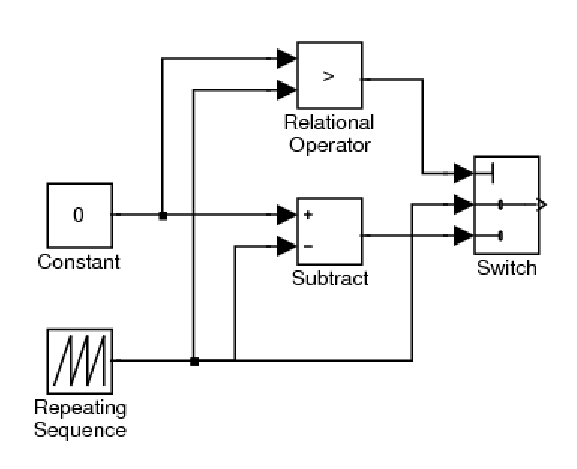
\includegraphics[scale=0.5]{figs/abs_simulink}
\caption{A Simulink model to compute the absolute value of an input}
\label{fig:abs_simulink}
\end{figure}

One of the major advantages of using Simulink, and also SCADE Suite,
is that it allows the hierarchical description of systems, enabling
top-down development. The building block for this hierarchical
description capability is a \emph{subsystem}. A subsystem, once
defined, can be instantiated within a system (or another subsystem),
assigned a rate, and its ports connected to various flows in the
containing system or subsystem. A subsystem's implementation contains
references to the ports it has defined, and internally its
functionality can be built up using either basic Simulink blocks, or
instantiations of still other subsystems. A system can thus contain
constituent subsystems, each of which may either be a user-defined
subsystem, or come from one of the many domain-specific ``libraries''
provided with Simulink. This helps in reuse of portions of the system
already developed. An example of this is shown in
Fig.~\ref{fig:subsystem_simulink} where the previous absolute value
logic is implemented in a subsystem (left part of the figure) and is
then used in a system as a building block (right part of the
figure). The susbsystem definition (left) contains references to the
ports \texttt{Abs\_In} and \texttt{Abs\_Out} that are shown connected
to the repeating sequence block and the graph block in the system
declaration (left), in this sense, ports may be considered to be the
formal and actual parameters of the subsystems.

\begin{figure}
\centering
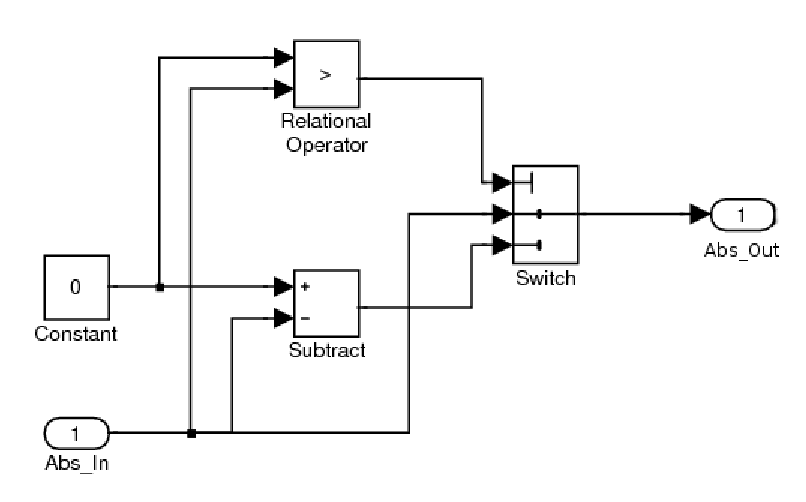
\includegraphics[scale=0.5]{figs/abs_block_simulink}
\hspace{10mm}
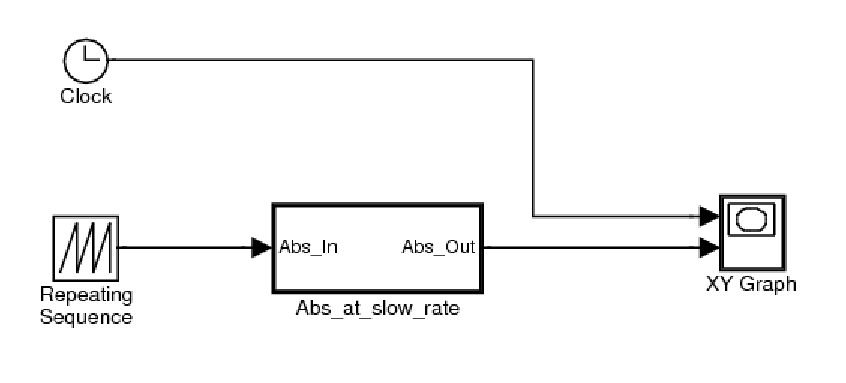
\includegraphics[scale=0.5]{figs/subsystem_simulink}
\caption{Left: The absolute value logic defined as a subsystem,
  \texttt{Abs\_In} and \texttt{Abs\_Out} are the input/output
  ports. Right: The absolute value subsystem used as part of a system
  design, the input and output ports are connected to a source and a
  scope}
\label{fig:subsystem_simulink}
\end{figure}

As stated, every block and subsystem in a system might either inherit
its rate from a driving block, or it can declare its own rate. In the
case of single-task systems---i.e., fully synchronous systems---all
rates must be integer multiples of the base
rate. Fig.~\ref{fig:abs_output_graphs} shows the same absolute value
subsystem as above instantiated twice within the system. One instance
runs at the base rate of the system, while the other instance runs
twice as slow. The lower part of Fig.~\ref{fig:abs_output_graphs}
shows the output flow from both subsystems, the left part showing the
output flow from the base rate subsystem, the right part showing the
flow from the slower subsystem, which results in undersampling, as
only one sample in two from the input is sampled.

\begin{figure}
\centering
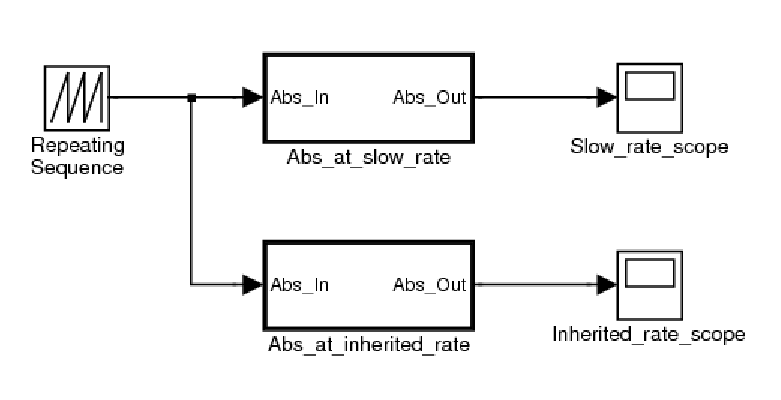
\includegraphics[scale=0.5]{figs/subsystem_rate_cmp_simulink}\\
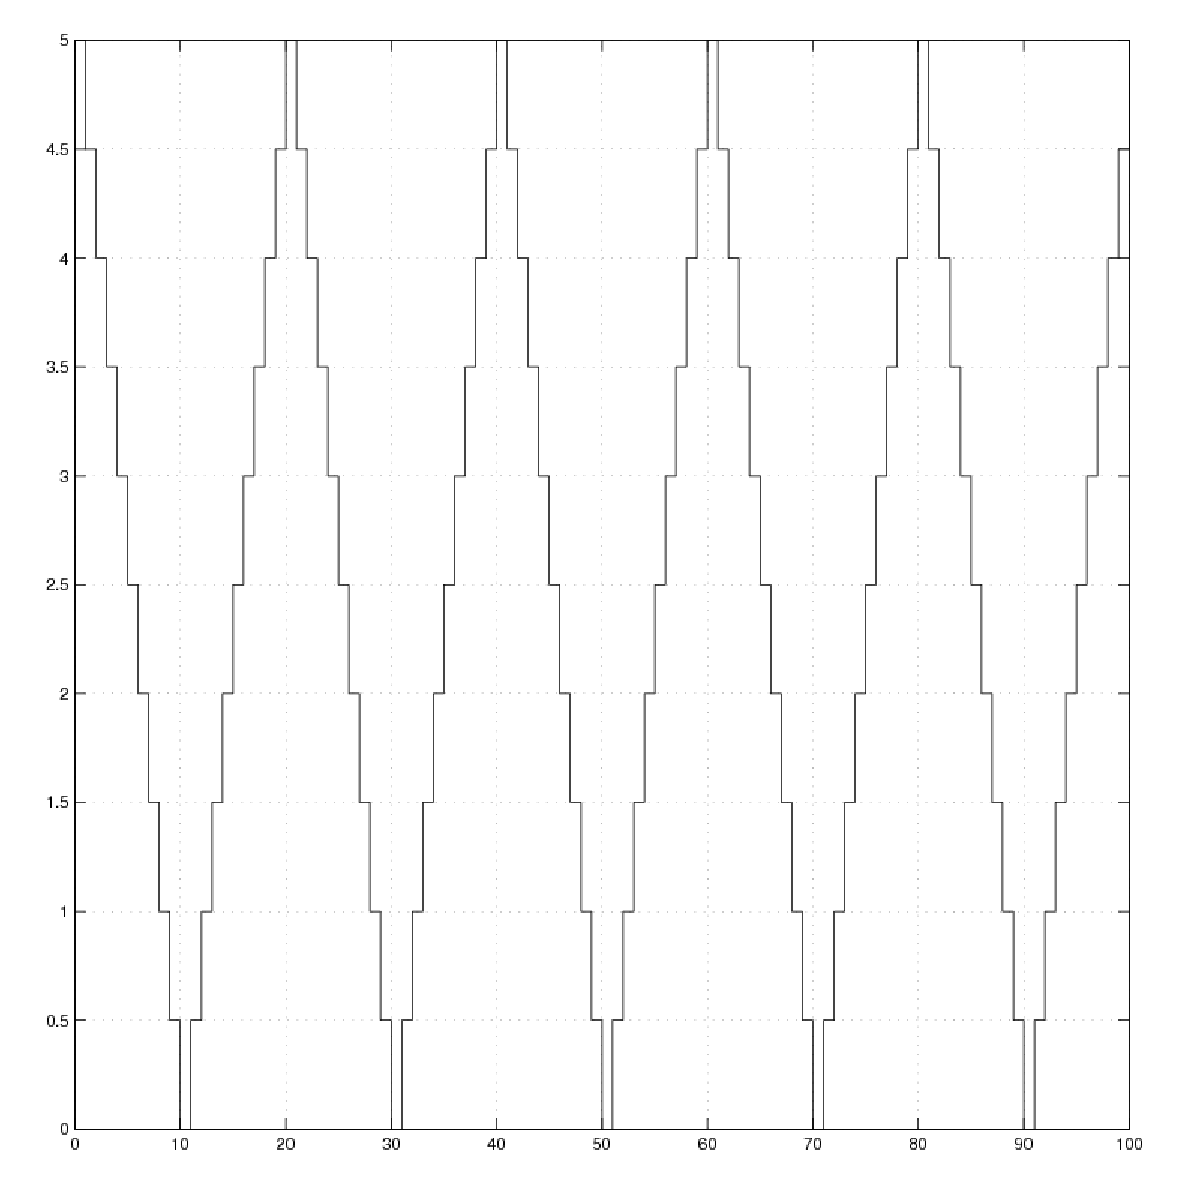
\includegraphics[scale=0.3]{figs/inherited_rate_scope}
\hspace{10mm}
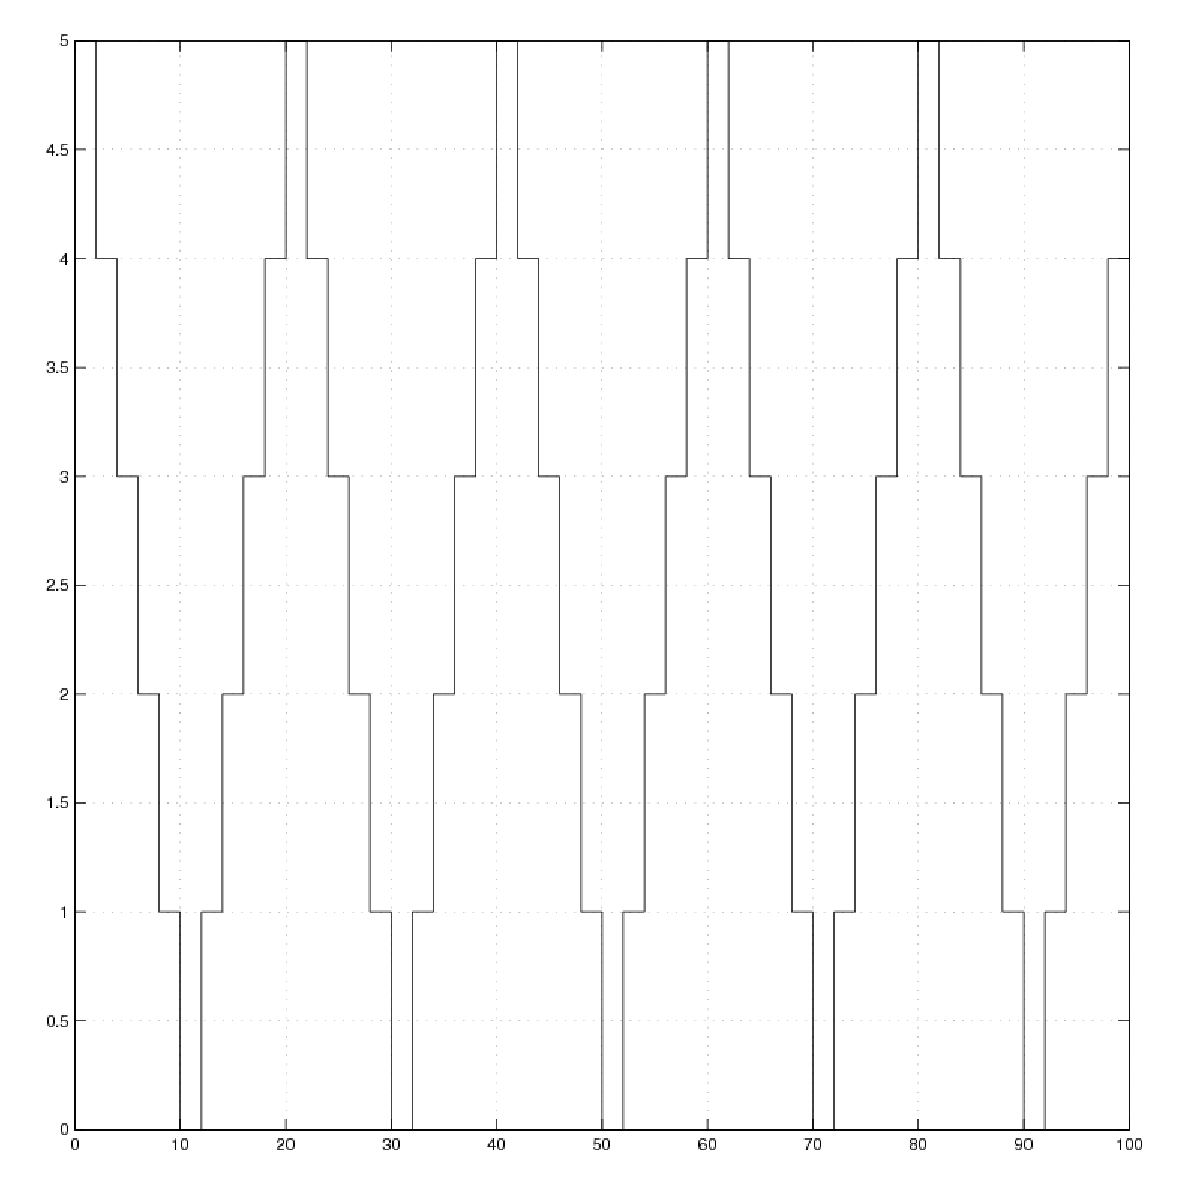
\includegraphics[scale=0.3]{figs/step_down_scope}
\caption{Above: Reuse of the absolute value subsystem, with two
  different instantiations, one running at the base rate of the
  system, the other one running twice as slow. Below left: the output
  from the subsystem running at the base rate of the system. Below
  right: The output from the subsystem running at half the base rate}
\label{fig:abs_output_graphs}
\end{figure}

The code generated from the single-task implementation is synchronous
and cyclic, thus the shared data variables that represent the various
ports and the flows traversing those ports need not be protected for
concurrency safe access. This is so because there is no concurrent
access, all blocks and subsystems are called in a linear sequence by
the timer interrupt, with the sequence being determined as a function
of the data dependencies among the blocks and subsystems, the topology
of the flows and the rates of the various blocks and subsystems. This
statically determined order of execution of the various blocks results
in a completely deterministic execution as well, with the resulting
determinism in data transfers among different blocks. The---C
programming language---function for each block is run completely
before that for another block is invoked. This implementation, like
all synchronous system models, assumes a zero-time execution
semantics, and brings all the prerequisite hypotheses and resulting
rigidity to the system.

The code generated for the multi-task implementations, on the other
hand, must be run on top of a real-time operating system. It uses OS
specific APIs to create and manage threads for the blocks and
subsystems running at different rates. This complicates the static
analysis of the execution order of the various blocks, as well as
introducing the possibility of race conditions in the access for
shared data representing ports. Thus, in a multi-task implementation,
the shared data buffers need to be protected via mutexes, and certain
buffer management techniques need to be used in case deterministic
data exchange between blocks at different rates is required.

The prevalence of Simulink in the control system design domain is
widespread. Tools exist to automatically translate a ``safe'' subset
of Simulink models~\cite{caspi@emsoft04} to
Lustre/SCADE~\cite{caspi@sigplan03}, as well as translations to the Z
formal description language~\cite{arthan@icfem00}. It has been
successfully used in the industry for applications such as automated
landing systems for UAVs\footnote{Boeing X40A}, cruise
control\footnote{Mercedes-Benz trucks} and computer-controlled braking
systems\footnote{Pacifica Group Technologies}.

\paragraph{Advantages of MATLAB Simulink}
\begin{itemize}
\item{It allows high-level modeling of control systems using a
  paradigm and notations familiar to engineers of the domain;}
\item{It allows code generation for a wide variety of operating
  systems as well as a bare bones target;}
\item{It contains a large number of pre-defined subsystems and blocks
  declared in different libraries, which furnish solutions to common
  domain problems;}
\item{It allows the generation of a synchronous system running on a
  cyclic executive, as well as a multi-task system running on top of a
  real-time operating system;}
\item{The extensive simulation capability of the tool provides the
  possibility of model-level debugging.}
\end{itemize}

\paragraph{Disadvantages of MATLAB Simulink}
\begin{itemize}
\item{It is principally suited to real-time control systems, as is
  evidenced by the fact that most of the blocks types available are a
  reflection of what is used in control system theory, e.g.,
  zero-crossing detection, integrators, zero-order holding, transfer
  function and zero-pole;}
\item{Its greatest strength---being close to the control system
  engineering domain---is also its greatest weakness. Because of its
  specificity, and the absence of pure computation artifacts, it is
  not very useful to the development of general real-time systems,
  which require the easy representation of computation steps such as
  loops, conditions, the sending of events and signaling among
  different tasks (just as it is counter-intuitive to develop control
  systems using software engineering concepts, it is counter-intuitive
  to develop generic software using control systems concepts);}
\item{Compared to SCADE Suite, Simulink does \emph{not} generate
  DO-178B certified code, so all code generated needs to be certified
  independently for conformance.}
\end{itemize}

\subsection{Unified Modeling Language}
The version 2 of the Unified Modeling Language ~\cite{uml-infra,
  uml-super}, or UML2, is a software design language standardized by
the Object Management Group. It is a primarily graphical language for
the design of object oriented software that arose out of three older
object oriented design methodologies; Rumbaugh's Object Modeling
Technique (OMT)~\cite{bruegge@oopsla92}, the Booch Method of Grady
Booch~\cite{white-booch} and the Object Oriented Software Engineering
(OOSE) from Jacobson~\cite{jacobson-oose}.

The OMG has chosen to standardize the UML2 based on a meta-modeling
framework called the Meta-Object Facility~\cite{mof-std}, or MOF. A
meta-model is the ``model of a model'', in that it describes the set
of all possible correct models. The OMG has defined the MOF as a
common meta-model for a wide variety of modeling languages, e.g., the
UML2, the System Modeling Language (SysML)~\cite{sysml}, the Object
Constraint Language (OCL)~\cite{ocl} etc. The benefits of this
approach are that all OMG modeling languages have the same
terminology, building blocks and an XML serialization schema because
one is provided for the MOF, and gets specialized for each modeling
language. In fact, a meta-model can be considered to represent the
abstract syntax of the modeling language it describes.

According to the MOF-based conception of UML2, there are four levels
of models. The most abstract layer is the meta-meta-model, provided by
the MOF. An instantiation of this meta-meta-model is the meta-model
(the UML2 meta-model in this case), this meta-model describes the set
of \emph{all} syntactically well-formed UML2 models. An instantiation
of the UML2 meta-model is a UML2 model, the design of a system,
whereas an instantiation of that is an actual running system. These
levels are conventionally called M3 through M0 and are shown
graphically in Fig.~\ref{fig:mof}.

\begin{figure}
\centering
\includegraphics[scale=0.75]{figs/mof}
\caption{The OMG Meta-Object Facility levels}
\label{fig:mof}
\end{figure}

UML2 is a general purpose software design language, due to which the
standard language contains a large number of different diagrams (13 in
total). Some of these diagrams are for documentation, others are for
analysis and the rest for code generation. The most important diagrams
from the point-of-view of real-time systems and automatic code
generation are \emph{class diagrams} and \emph{statecharts}.

A class diagram shows the relationships between the classes in a
system. It shows class hierarchies, associations and containments
among the various classes of the system. In addition, it can show the
internals of these classes, such as their attributes and member
functions, as well as access specifiers on said attributes and member
functions (protected, private or public). The class diagram is the
basic unit for code generation of a system, since it is where class
specifications are given. The main relationships among classes that
can be given in class diagrams are:

\begin{description}
\item[Inheritance:]{Specifies that one class inherits from another;}
\item[Association:]{Specifies that objects of one class have link(s)
  to object(s) of another class and allows navigation from the source
  object to the object(s) of the class pointed to as each association
  corresponds to having a reference(s) for the objects to which the
  association points;}
\item[Composition:]{Specifies that an object of one class contains one
  or more objects of another class.}
\end{description}

Fig.~\ref{fig:class_diag} shows a class diagram for an imaginary
automotive control application. \texttt{RPM\_Controller} is a class
derived from \texttt{Valve\_Controller}, the thicker edges of
\texttt{RPM\_Controller} and \texttt{Driver\_Input} signify that they
are \emph{active} classes, i.e., they have their own threads of
control. Both have an association to \texttt{Driver\_Params}, which in
this case represents a shared data buffer with accessor methods. The
object of class \texttt{Driver\_Input} contains one object each of
\texttt{Accelerator\_IO} and \texttt{Brake\_IO}, which is represented
via the composition relation. The generated code for this object model
would contain threads for the two active classes. It would also
contain the shared buffer's code which would comprise the declared
attributes as data members and member functions with the correct
signatures.

\begin{figure}
\centering
\includegraphics[scale=0.75]{figs/class_diag}
\caption{A class diagram showing various types of relations among
  classes allowed in UML, made using Rhapsody}
\label{fig:class_diag}
\end{figure}

The other major diagram within UML2 which aids greatly in real-time
systems development is the Statechart~\cite{jansamak@acsc04,
  allen@sigplan95}. Statecharts are state machine diagrams that can be
attached to active classes to describe their behavior. Statecharts are
a form of extended input output automata~\cite{lynch@concur01} which
can access and modify the attributes of the class they are attached to
and can send \emph{signals}---asynchronous events---to other active
classes with statecharts attached. An example of a statechart diagram
is shown in Fig.~\ref{fig:statechart}, it is a state machine that
implements the behavior of a hypothetical water heater that can heat a
sample of water up to a desired temperature.

\begin{figure}
\centering
\includegraphics[scale=0.5]{figs/statechart}
\caption{A UML statechart diagram, attached to a class to describe its
  behavior}
\label{fig:statechart}
\end{figure}

With these capabilities, UML2 is used quite extensively within the
real-time and vehicular control industries for modeling and design of
software systems. CASE tools such as Rhapsody$\circledR$ provide
capabilities of code generation, which reduces time spent in software
development because the behavior of the system can be simulated at the
level of the model rather than at the level of source code, this
coarse-grained debugging exercise results in catching of conceptual
errors earlier in the design process than would be possible if the
application had been coded by hand.

That said, there are some disadvantages to using UML2 for the design
of safety-critical real-time systems. The language is very large and
complex, the three main documents of the language
definition~\cite{mof-std, uml-infra, uml-super} together make for over
2,000 pages. The semantics of the language is not formally defined,
leading to different tool vendors implementing their own
interpretation of the constructs. Neither of these disadvantages,
however, is as great as the fact that the language itself is not
geared towards the design of real-time systems. Case in point is the
concept of active classes; they represent threads in the generated
code, however there is no concept of periodic active class, aperiodic
active class or sporadic active class. There are no concepts of
deadline, worst-case execution time or even priority. The system and
software designer is expected to cater to those requirements
himself. This, compounded with the fact that the entire concept of
using separate notations of the same basic artifact (a class) for
different runtime entities is an indication of semantic overloading in
the language definition. Thus, even though UML2 \emph{is} used within
industry for the modeling and design of real-time systems, it is not
extensively used for hard real-time systems, rather mostly for soft
real-time systems and/or monitor and alarm subsystems.

\paragraph{Advantages of UML}
\begin{itemize}
\item{It is now a standardized language, and it is very prevalent in
  the software industry, expertise in UML is relatively widespread;}
\item{It is a modeling language that is close to the software domain,
  this can be seen as an advantage (from the software developer's
  point-of-view) or as a disadvantage (from the system engineer's
  point-of-view);}
\item{It is a language that allows the modeling of object oriented
  concepts and artifacts, together with the integration of functional
  aspects or behavioral descriptions (in the form of Statecharts) in
  the same model;}
\item{It has a reasonably intuitive conversion to source code,
  specially in an object oriented language such as C++ or Java, i.e.,
  the vertical distance for a transformation to source code is small;}
\item{Since all implementations of UML are supposedly based on the
  MOF, model storage is done via a standardized XML serialization and
  in theory models can be interchanged between tools;}
\item{It contains extensibility mechanisms built into the language via
  the stereotype mechanism.}
\end{itemize}

\paragraph{Disadvantages of UML}
\begin{itemize}
\item{There are no formal semantics of the language, therefore, the
  interpretation of the language standard leaves a lot of leeway to
  the individual tool developer. This results in the people being
  experts not of UML, but of a certain UML IDE;}
\item{The language is very complex. The standards documents together
  make up about 2000 pages, and the language has 13 different diagram
  types;}
\item{It is very strongly tied to the object oriented languages. In
  fact it can be viewed as a graphical methodology to the design of
  object oriented programs. Real-time systems often eschew object
  orientation in favor of deterministic execution times;}
\item{UML forces \emph{semantic overload} on the basic artifacts of
  UML to represent new concepts. As an example consider that an active
  class in UML is considered to be a thread of execution, instead of
  being a class, this type of semantic overload introduces confusion
  in the model.}
\end{itemize}

\subsection{HRT-HOOD and HRT-UML}
The Hierarchical Object Oriented Design
methodology~\cite{vielcanet@wadas89} was a design technique developed
in the mid 80s for the design of aerospace software under contract by
the European Space Agency. Its next version, specifically for
real-time systems, is HRT-HOOD (Hard Real-Time
HOOD)~\cite{burns@rts94}, which contains specific artifacts and
constructs for real-time systems, which eases timing analysis and
leads to a safer design. HRT-HOOD allows the modeling of real-time
systems using one of five types of objects:

\begin{description}
\item[Passive objects:]{These are objects that do not have their own
  thread of control nor do they invoke operations on other objects;}
\item[Active objects:]{These objects may control when invocations of
  their operations are executed---they have a thread of control---and
  they can invoke operations of other objects;}
\item[Protected objects:]{These are objects that may control when
  invocations of their operations are executed (via the enforcement of
  a concurrency control protocol). Protected objects must also be
  analyzable for the blocking time they impose upon calling objects;}
\item[Cyclic objects:]{These are objects which represent periodic
  threads. They may call operations in other objects;}
\item[Sporadic objects:]{These are objects which represent sporadic
  threads.}
\end{description}

Because HRT-HOOD is a hierarchical description technique, objects
defined using it may be non-terminal objects, which contain other
objects, or terminal objects, which may be of one of the previously
described types. Non-terminal objects may receive requests, which are
delegated to the contained objects to be treated.

All types of objects may expose operations. However, there are
constraints on the types of operations the various types of objects
may expose. A passive object exposes operations that have no
synchronization constraints, they are executed as soon as they are
invoked, and their execution takes place in the context of the
caller's thread. Thus a passive object is like a normal object in an
object oriented language or a module in a structured language. An
active object's operations may be constrained or unconstrained, they
may be executed immediately upon invocation or may require
synchronization and access control, furthermore, an active object may
or may not have its own thread of control (active objects were removed
in the next version, called HRT-UML). Passive objects, as they are
used to provide concurrency-safe access to shared resources, may
expose two types of operations; \emph{protected synchronous execution
  requests} (PSER) and \emph{protected asynchronous execution
  requests} (PAER). PSERs can make the calling object wait for a
condition to become true in addition to enforcing mutual exclusion
(they are like condition variables), whereas PAERs implement simple
mutual exclusion (they are like mutexes). Cyclic objects do not have
operations defined on themselves, however they may call operations on
passive objects in order to exchange data with other objects. In
certain cases a cyclic object may have an associated protected object,
which is used to send data to the cyclic object. Such a protected
object is called the OBCS (Object Control Block Structure) of the
cyclic object. A cyclic object will also have a passive object
associated to it, which is called its OPCS (OPeration Control
Structure). The OPCS is the functional unit of the cyclic object,
i.e., it is where the periodic response code of the cyclic object is
found, and it is this part of the cyclic object that is written by
hand. Sporadic objects must necessarily have an OBCS associated, upon
whose only PSER operation the sporadic object will wait for
dispatch. A sporadic object also has an OPCS which represents its
response to the various dispatching events.

These objects may have associated with them various \emph{attributes},
which represent their configuration and/or code generation
parameters. Examples of important attributes include DEADLINE,
THREAD\_WCET, PERIOD, MINIMUM\_ARRIVAL\_TIME and PRIORITY for cyclic
and sporadic objects. Some of these attributes are to be assigned by
the designer while others are calculated as a function of the system
architecture by the code generator.

HRT-UML~\cite{mazzini@ae03} is the latest version of this
methodology. It removes certain unsafe constructs present in HRT-HOOD
and introduces the methodology as a \emph{profile} of UML, where the
artifacts of the language are shown as UML classes with specific
stereotypes. Furthermore, HRT-UML is targeted to the Ada Ravenscar
Profile for High-integrity systems~\cite{burns@adalett04} which is a
subset of Ada specifically tailored for high-integrity hard real-time
systems (detailed in Sec.~\ref{sec:rsp}). HRT-UML puts a high value on
the static schedulability analysis of systems described with it. There
has been research work done to incorporate automatic code generation
as well~\cite{vardanega@ecrts05}. A detailed case study using the
approach is given in~\cite{silvia-hrt-uml-cs}.

The HRT-UML firstly removes the active objects from the HRT-HOOD,
since they are not amenable to static analysis. Also not included in
this language are two operation invocation protocols from HRT-HOOD
called the \emph{loosely synchronous execution request} (LSER) and the
\emph{highly synchronous execution request} (HSER) because they both
required two separate threads to synchronize with each other, which
leads to unpredictable execution times and thus impacts the static
analyzability of the system.

Since HRT-UML is a UML profile, the various objects are declared as
UML objects with the appropriate stereotypes. In this case the
stereotypes being $\ll periodic\gg$, $\ll sporadic\gg$, $\ll
protected\gg$ and $\ll passive\gg$. The above-mentioned attributes of
the objects become the meta-attributes of the stereotypes
defined. Thus, e.g., classes with the stereotype $\ll periodic\gg$
will have meta-attributes DEADLINE, PERIOD and PRIORITY, which will be
processed or generated by the tool.

\paragraph{Advantages of HRT-UML}
\begin{itemize}
\item{It allows the explicit modeling of software constructs relevant
  to the hard real-time domain, i.e., periodic and sporadic objects;}
\item{The real-time systems attributes of these constructs are
  intuitively given and readily observable, i.e., period, priority,
  minimum interarrival time etc.;}
\item{It \emph{folds} the design method into UML, which is the
  emerging omnipotent vehicle for software design. This could
  potentially allow the description of the real-time system
  architecture (via HRT-UML constructs) alongside the software design
  of the response code in the shape of class diagrams for the OPCS
  portions;}
\item{It also allows for the functional description of the system
  using UML Statecharts;}
\item{It allows for static schedulability analysis via the Rate
  Monotonic and Response Time analyses;}
\item{It allows for automatic code generation, greatly reducing
  programmer effort and chance for error.}
\end{itemize}

\paragraph{Disadvantages of HRT-UML}
\begin{itemize}
\item{Its greatest strength may also be seen as a weakness, i.e., it
  uses UML, which is a large and rather unwieldy standard/language;}
\item{It engages in semantic overload even more than basic UML. Where
  basic UML only says an active class is a thread, HRT-UML overloads
  the notion by saying it may be periodic or sporadic;}
\item{It forces the designer to model the application at a very fine
  grain, i.e., very near to the runtime artifacts that will exist. In
  fact, HRT-UML may be considered a graphical representation of the
  concepts of the Ada tasking model. It shows all synchronization and
  communication buffers as part of the model rather than abstracting
  them out (e.g., in the case of Simulink they are abstracted out as
  ports), this results in model clutter and distracts from the
  domain-specific exercise of modeling.}
\end{itemize}

\subsection{MARTE UML2 Profile}
There is yet another UML2 profile that seeks to model distributed,
real-time embedded systems. This profile, named MARTE (Modeling and
Analysis of Real-Time and Embedded systems) is an OMG
standard~\cite{omg-marte}. It uses a mechanism similar to that for
HRT-UML for describing various real-time aspects of the system it is
used to model, in that it makes extensive use of the stereotype
construct to add semantic information to a UML class. This semantic
information can be parsed and understood by a tool that is familiar
with the conventions in the profile.

This profile contains not only notation support for real-time systems,
but also extensive support for QoS and dependability
measures~\cite{bernardi@wosp07}. There is also a proposal to use the
MARTE Profile as a means of modeling systems in the AADL---the
architecture description language used as a starting point for the
research presented in this thesis---by creating a mapping from MARTE
to AADL~\cite{gerard@iceccs07}. This profile brings the same
advantages and suffers from the same disadvantages as the HRT-UML
profile discussed above, however, there are some differences which are
pointed out below:

\paragraph{Advantages of MARTE}
\begin{itemize}
\item{It is an extensive profile, it contains a myriad of modeling
  possibilities. The user can model the temporal characteristics of
  the system, the QoS and dependability properties, the resource usage
  in terms of memory and processing power as well as electrical
  consumption etc.;}
\item{It is an OMG standard, which gives it a visibility and
  credibility not afforded to other, lesser-known or lesser-sponsored
  methodologies;}
\item{There is rudimentary tool support, in the form of the open
  source Papyrus UML tool\footnote{Available at
    \url{http://www.papyrusuml.org/}}.}
\end{itemize}
\paragraph{Disadvantages of MARTE}
\begin{itemize}
\item{Again, its biggest strength is also its weakness. It takes on so
  much functionality that it is now suffering feature bloat;}
\item{It presents a very steep learning curve due to its complexity;}
\item{There is no concrete effort---at least not yet---towards
  automatic code generation from MARTE models, it is currently only
  used for analysis purposes.}
\end{itemize}

\subsection{MetaH}
MetaH is an architecture description language originally developed by
the Honeywell Advanced Technology Center for use in avionics
systems~\cite{metah-manual}. It is also the direct ancestor of the
AADL, which is the architecture design language used in the research
work being presented. MetaH, like other ADLs, focuses more on software
architecture than on software design. It contains entities that
correspond to what may be viewed as high-level runtime constructs such
as threads, communication buffers and modules rather than software
design concerns such as classes, objects and their
interrelations. Thus, like other ADLs it focuses on component
interfaces, properties and connection topology rather than their
internals. The MetaH toolset from Honeywell includes a graphical
modeler, schedulability analyzer for the system model, a code
generator for C and Ada as well as a real-time executive that can run
the generated application.

MetaH is a component-centric ADL that contains the facilities for the
definition of the hardware setup atop which the software entities it
defines will execute. The hardware components of MetaH are processor,
memory, device and channel. These hardware components can be used to
describe the overall hardware configuration of the system under
consideration, e.g., the designer can specify that a system consists
of two processors linked together via a channel; the software
components of MetaH can then be declared to be hosted on one of the
two processors. The software component categories supported by MetaH
include process, event, port, type (in the sense of data type), type
package, monitor, subprogram and package. A real-time executive exists
which provides APIs and facilities to host and execute applications
generated from MetaH models.

\begin{description}
\item[Process:]{It is the basic unit of execution and schedulability
  (no threads in MetaH). A process may be periodic or aperiodic;}
\item[Event:]{It is an asynchronous signal sent to a process. Events
  are used to dispatch aperiodic processes;}
\item[Ports:]{These are data transfer endpoints declared in the
  interface of a process. Ports are typed and serve as message buffers
  between processes, they also have directional qualifiers \textbf{in}
  and \textbf{out}. The executive provides real-time data transfer
  facilities to implement ports;}
\item[Package:]{It is a collection of data objects and procedures that
  can act upon those objects. It can be used to give a rudimentary
  software design for the functional response code of processes;}
\item[Monitor:]{It is similar to a package except that it may be
  accessed by multiple processes, hence it requires concurrency
  control, which is ensured via the use of real-time semaphores
  provided in the MetaH executive;}
\item[Processor:]{It represents a CPU, processes are declared as being
  bound to a processor component;}
\item[Memory:]{It represents a random access memory;}
\item[Device:]{It represents any specialized hardware that cannot host
  user-defined software but that may send or receive events and data
  to the user-defined software. Device components are mainly used to
  provide a model-level abstraction of sensors, actuators and other
  hardware;}
\item[Channel:]{It is a hardware entity that connects various other
  hardware components together and provides a path for data and/or
  event transfer among them.}
\end{description}

MetaH is geared towards the development of control systems. In this
respect, its port construct is similar to that found in Simulink,
i.e.: a port is a \emph{state}. This means that a port cannot contain
a queue, and in fact according to the coding guidelines each port on a
process interface is simply transformed to a static variable. At
runtime, values in the variables corresponding to \textbf{out} ports
are automatically transferred to the variables corresponding to the
\textbf{in} port(s) to which they are connected. Thus, ports, and the
variables they are transformed to, can be viewed as data flows, which
meshes well with the nature of control laws and their implementations.

Events in MetaH are pure signals that can be used to dispatch
aperiodic threads. Events may not contain any accompanying data. In
source code, an event reception is transformed to a blocking call of a
procedure of the executive, in this case called
\texttt{Await\_Dispatch}, which also returns an enumeration to denote
the event type that was received. A call to this procedure is a part
of the response code of each aperiodic thread. The return from this
procedure is the semantic equivalent of the reception of the event. On
the sender's side, the corresponding procedure is called
\texttt{Raise\_Event} and may be used by the functional response code
of any process to send an event to another, provided there is a pair
of connected event ports with the appropriate directional qualifiers
between the two.

MetaH includes a system of attributes, which are name/value pairs that
can be assigned to various components for aspects of their design or
configuration parameters that cannot be expressed otherwise. Examples
of attributes include \texttt{Period}, \texttt{Deadline} and
\texttt{Criticality} for process components; \texttt{SourceName} for
ports and \texttt{SourceFile} for package components.

MetaH is interesting because it provides an attractive level of
abstraction for real-time system implementation. The abstraction level
is not as high as Lustre or Simulink, since software artifacts such as
processes, shared variables etc. are visible in the model. But the
abstraction level is not as low as UML or HRT-UML either, in that the
presence of the port construct allows the hiding of data flow
buffers. This results in a concise and uncluttered model when data
flow applications are being designed, yet retains the flexibility of
describing sophisticated shared data buffers if and when their need
arises, via the use of the monitor construct. The port construct,
though it may seem rather trivial, is an important capability. It
allows for a concise description of the data flow within the system,
\emph{and} it can be used to embed protocol information in the system
model. This capability is used to model deterministic data flow
connectors as shown in Chapter~\ref{chap:adv_code}.

\paragraph{Advantages of MetaH}
\begin{itemize}
\item{Provides a concise, clear and unambiguous set of constructs for
  modeling real-time systems;}
\item{Inclusion of hardware components allows system models with the
  hardware and software architecture in the same model. This aids in
  analysis and code generation for distributed applications;}
\item{The port construct allows an intuitive modeling of data flow
  applications, which aids in the design of control systems by letting
  the modeling reflect domain space.}
\end{itemize}

\paragraph{Disadvantages of MetaH}
\begin{itemize}
\item{The absence of threads precludes modeling of multithreaded
  applications. One process is one partition and can only contain one
  unit of execution and schedulability;}
\item{The technology is proprietary and not open to modification;}
\item{Allows for aperiodic threads, which are unsafe as they may lead
  to system overload;}
\item{Event ports may not have associated data, this makes it
  difficult to implement general real-time systems, i.e., other than
  control systems;}
\item{The attributes of each type of component are fixed, new
  attributes cannot be defined. This restriction of extensibility
  precludes any additional information being added to the model than
  was originally designed.}
\end{itemize}

\section{Conclusions}
This chapter has put in context some of the current practices in
real-time systems development, from a number of different
points-of-view. It has provided an introduction to the domains of
real-time tasks \emph{and} real-time schedulers. The clarification
between a cyclic executive and a process-based executive has been
given, and the theoretical and practical implications of the choice of
each have been enunciated. The various model driven code generation
approaches for real-time systems have been presented, along with
advantages and disadvantages for each. Here, it bears stating that
even though disadvantages for each approach have been provided, it is
by no means being claimed that \emph{any} of these approaches is
useless or not used. As a matter of fact, the approaches mentioned
were discussed for the reason that they \emph{are} widely
used. Lustre/SCADE Suite is the tool used to develop the fly-by-wire
systems of all modern aircraft from Airbus Industrie, as well as
nuclear reactor control software from Schneider Electric. \simu is
widely used in the US aerospace industry for similar purposes
(fly-by-wire systems design). The UML is the most widely used software
design language in the general market, and it is also extensively used
within the real-time systems community.

%%% Local Variables:
%%% mode: latex
%%% mode: flyspell
%%% TeX-master: t
%%% End:
